\documentclass[../Maxima_Workbook.tex]{subfiles}

\begin{document}
	
\chapter{Coordinate systems and transformations}

\section{Cartesian coordinates}

\subsection{Extended coordinates}

\lz \hyt{Leng}{\tcr{\emph{Leng ($ \gpal vector \; \gbar \; square matrix \gpar $, $ \glangle 1 \gbar 0 \grangle $)}}} \hfill \tcr{[function of \emph{rs\_object\_transformation}]}\index{Leng} \\
\hyt{Short}{\tcr{\emph{Short ($ \gpal vector \; \gbar \; square matrix \gpar $)}}} \hfill \tcr{[function of \emph{rs\_object\_transformation}]}\index{Short}

\lz Function \emph{Leng} transforms a column vector or square matrix of dimension 2 or 3 to extended coordinates. If the first argument is a column vector, add a new component at the end containing 1 for a location vector and 0 for a direction vector, depending on the optional second argument (1 or 0). If the second argument is omitted, use 1, since a location vector is assumed. A column vector is returned. In case of a square matrix, 0 is appended to any column and row, only the last element of the matrix is set to 1.

\lz The inverse function \emph{Short} transforms a column vector or square matrix of dimension 2 or 3 being in extended coordinates (dimension 3 or 4) back to the non-extended format.

\subsection{Object transformation}

\subsubsection{Rotation}

\lz \hyt{RotMatrix}{\tcr{\emph{RotMatrix ($ \gpal 2D \; \gbar \; axis \gpar $, phi, $ \glangle extend \grangle $)}}} \hfill \tcr{[function of \emph{rs\_object\_transformation}]}\index{RotMatrix}

\lz Returns the rotation matrix (in extended coordinates, if 3. argument is present, e.g. as \emph{e}) for an active (object) rotation in 2D, if first argument is \emph{2}, else in 3D around axis \emph{x}, \emph{y}, or \emph{z}, with rotation angle \emph{phi} (given in rad) in the mathematically positive direction (counterclockwise). By giving a negative angle $ - $\emph{phi}, the transformation matrix for a passive (coordinate) rotation in the mathematically positive direction (counterclockwise) by angle \emph{phi} can be created.

\section{Polar coordinates}

\section{Cylindrical coordinates}

\begin{SCfigure}[0.33][h]
	\centering
	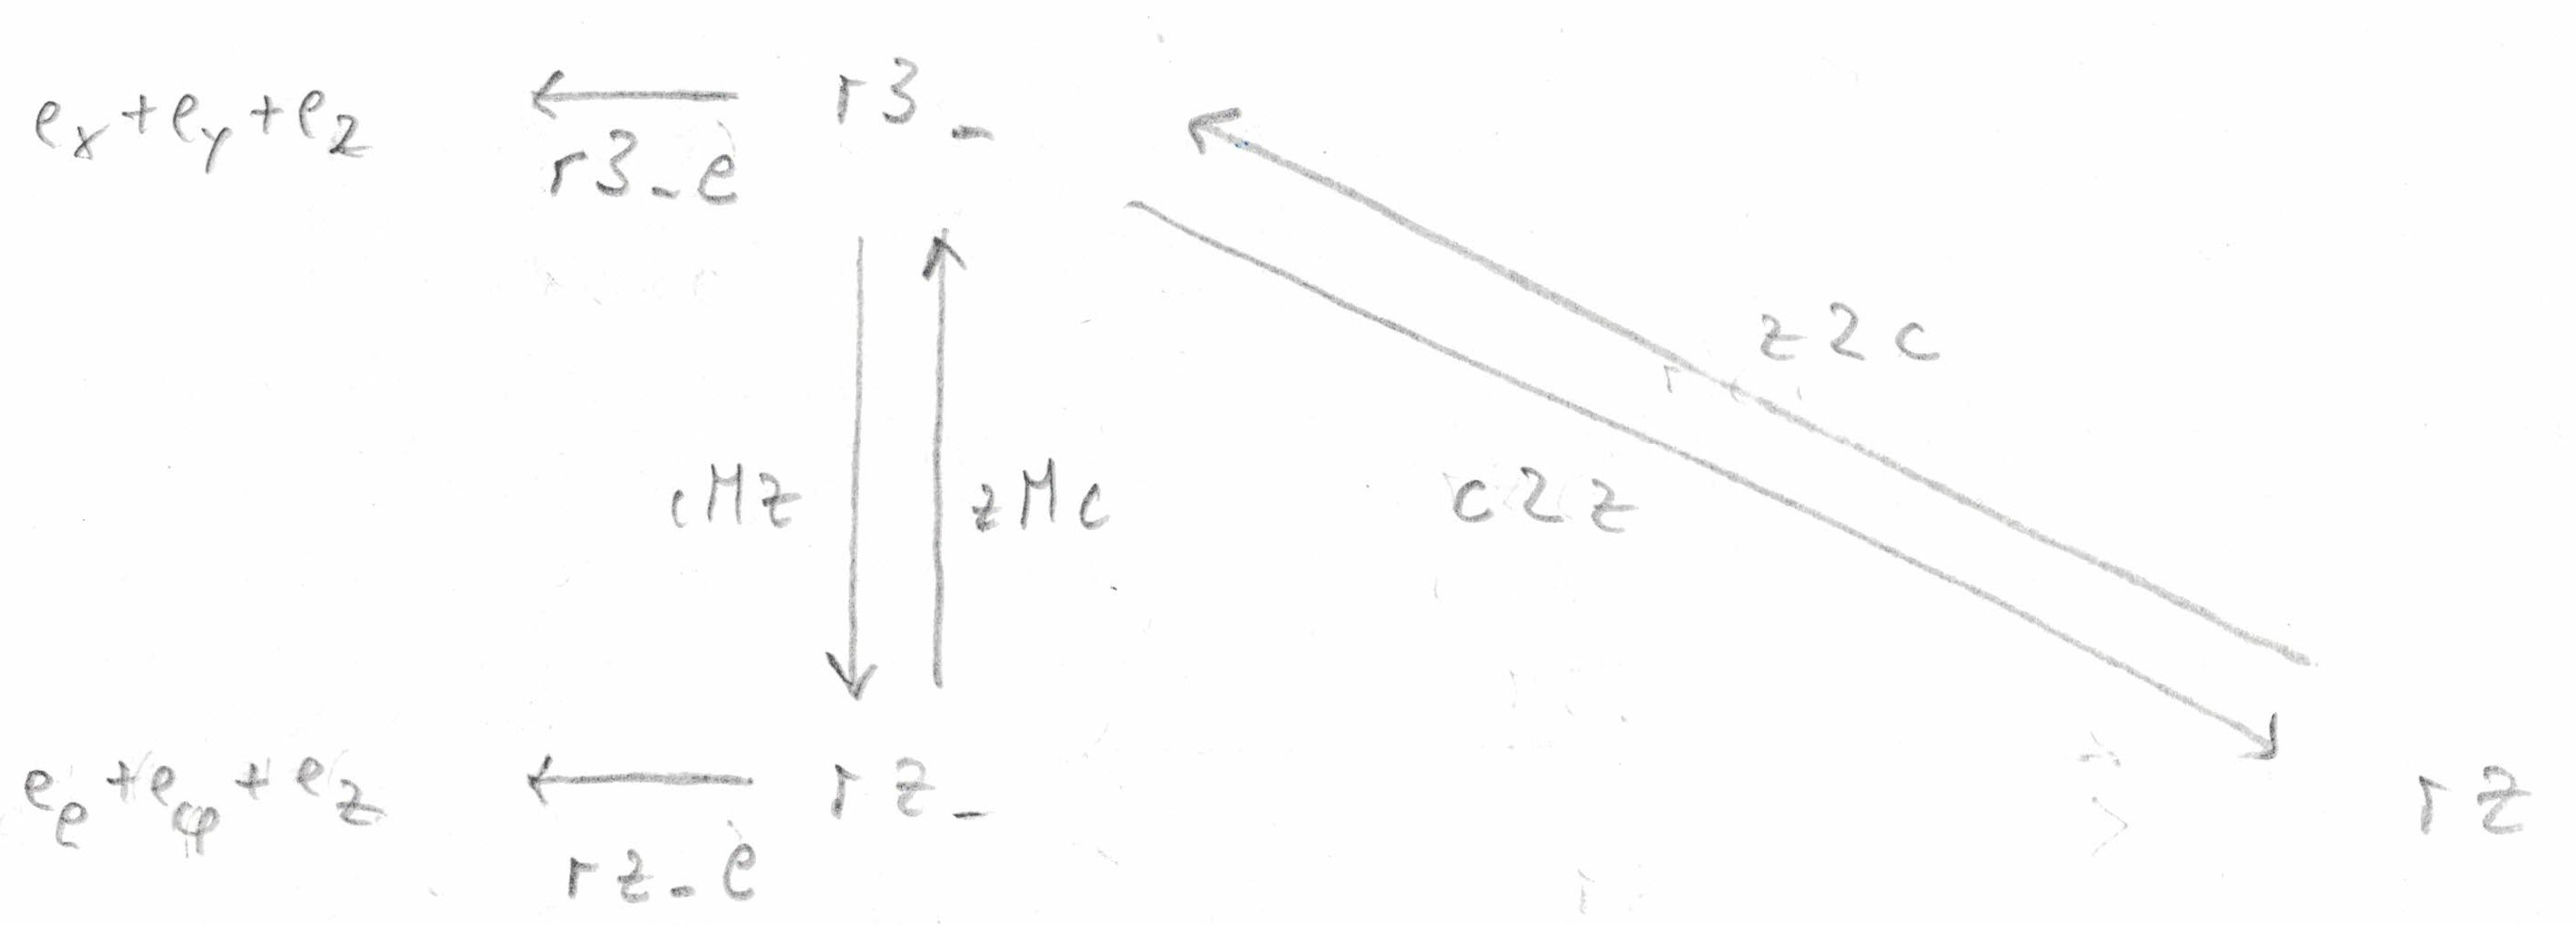
\includegraphics[width=0.75\textwidth]{CS-Fig1.jpg}
	\caption{Diagram of representations and transformation functions for cylindrical coordinates from package cylindrical\_coordinates.mac.}
	\label{CS-Fig1}
\end{SCfigure}

\section{Spherical coordinates}

\section{General orthogonal coordinates}

\end{document}